% -*- coding: utf-8 -*-


\cleardoublepage
\plainifnotempty


\chapter{データベースシステムの夜明け}


\begin{flushright}
はやみず
\end{flushright}


\lettrine{デ} \ \ ータベースシステム無しでは,今日の社会は成り立たないと
言って良いでしょう。社会が高度に情報化された現在,世界中で大量のデジタル
データが日々生み出され,飛び交い,消費され,そして蓄積されてゆきます。一
方で,膨大なデジタルデータは,単に生み出され,蓄積されてゆくだけではゴミ
も同然です。必要なときに必要なデータが取り出せるよう,適切に管理してゆか
なければなりません。そのための根幹たる存在がデータベースシステムなのです。


今日においては,「データベースシステム」と呼ばれているその殆どが「リレー
ショナルデータベースシステム」です。みなさんが馴染みのあるであろう MySQL
や PostgreSQL,あるいは Oracle といったデータベースシステムは,すべてリレー
ショナルデータベースシステムですね。リレーショナルデータベースシステ
ムの歴史を辿ると,その起源はある一篇の論文に遡ることができます。


その論文こそが,Edgar F.  Coddにより1970年に発表された ``A Relational
Model of Data for Large Shared Data Banks'' です。この論文は,リレーショ
ナルデータベースの最も重要な基礎となる{\bf リレーショナルモデル}を提唱し
たもので,いわばデータベースシステム分野における金字塔です。古典力学を
Newton が拓き,相対性理論を Einstein が拓いたとするならば,データベースの
一大分野であるリレーショナルデータベースを拓いたのは Edgar F. Codd その人
といって間違いないでしょう。


データモデルとは,どのような形式でデータを格納して,どのようにデータにア
クセスするかということを取り決める枠組みです。データを蓄積・管理することを目
的とするデータベースシステムにおいては,データモデルはその心臓部とも言え
る存在なのです。


そして,Codd によるリレーショナルモデル提唱から数年の後に,UNIXで動作する
世界初のリレーショナルデータベースシステムの開発プロジェクトが立ち上がり
ます。Michael Stonebraker率いる{\bf INGRESプロジェクト}です。Coddにより確
立されたリレーショナルデータベースシステムの基礎理論を,実際に動くソフト
ウェアとして実現し,そしてそれを世に広めたのがINGRESなのです。


本稿では,Coddによるリレーショナルモデルの提唱から,INGRESプロジェ
クトの黎明期の記録を辿り,現代の社会を支えるデータベースシステムがいかに
して創り上げられたのか,その歴史を紐解いてみようと思います。


\section{リレーショナルモデルの登場}


リレーショナルモデルが登場する以前,つまり1960年代までのデータベースシス
テムは殆どが階層型モデルやネットワーク型モデルというデータモデルに基づい
て構築されていました。


\begin{figure}[tb]
 \begin{minipage}{0.48\textwidth}
  \begin{center}
   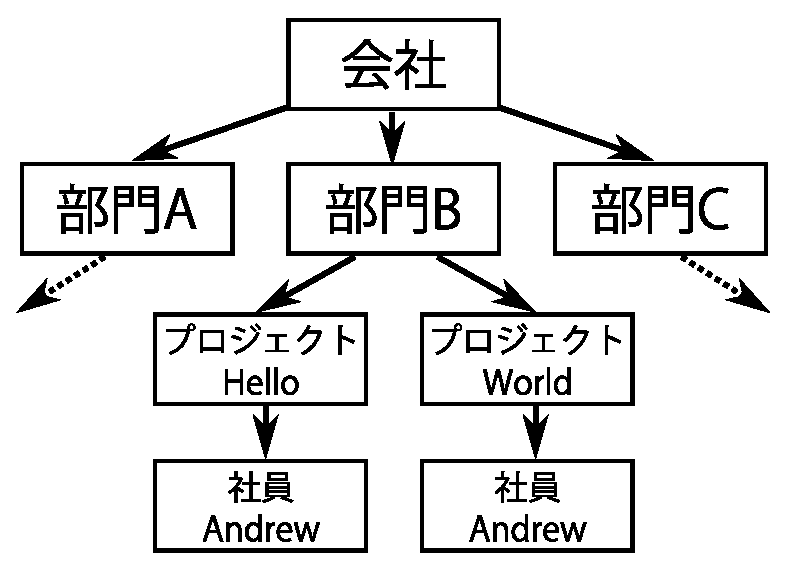
\includegraphics[width=5cm]{hayamiz/images/hierarchical-data-model.eps}
   \caption{階層型モデル}
   \label{214539_12Jul12}
  \end{center}
 \end{minipage}
 \begin{minipage}{0.48\textwidth}
  \begin{center}
   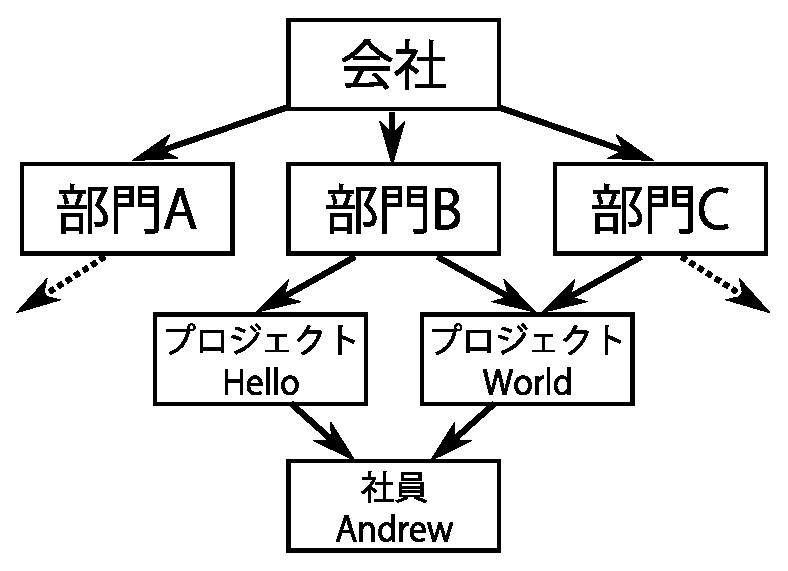
\includegraphics[width=5cm]{hayamiz/images/network-data-model.eps}
   \caption{ネットワーク型モデル}
   \label{214707_12Jul12}
  \end{center}
 \end{minipage}
 \vspace*{-0.1\Cvs}
\end{figure}


階層型モデルというのは,木構造を用いてデータを組織化したデータモデルです。
たとえば会社組織を階層型モデルで表すとしましょう。この会社では,会社の中
に複数の部門があります。各部門の中では複数のプロジェクトが運営されていま
す。そして各プロジェクトに従業員が属しています。そうすると,図
\ref{214539_12Jul12}のような階層構造でデータを組織化することができます。


ここで,例えば2つのプロジェクトHello projectとWorld projectに属する1人の社員Andrewがいた
としたらどうでしょう。階層型モデルにおいて,1つのデータの実体(社員やプロ
ジェクト)が複数の親データに属することができません。つまり,1人の社員が複
数のプロジェクトに属することを直接表現することができないのです。無理やり
これを表現しようとすると,各プロジェクトごとにAndrewのデータを持つことに
なり,データの重複が生じてしまいます。また,部門Bと部門Cが共同でプロジェ
クトWorldを運営していることを表現しようと思うと,プロジェクトのデータに加
えてその下にぶら下がっている社員のデータも併せてコピーしなければなりませ
ん。
階層型モデルは非常にシンプルで性能が出しやすいというメリットもあるのですが,このようにデータ同士の関
係を柔軟に記述することができないというデメリットもあるのです。


このような階層型モデルの欠点を克服したのがネットワーク型モデルです(図
\ref{214707_12Jul12})。ネットワーク型モデルでは,木構造ではなくグラフ構造
によりデータの組織化を行います。グラフ構造であれば Andrew が複数プロジェ
クトに属することを自然に表現できるために,前述のようなデータ重複の問題は
発生しません。


1960年代には,IBMによってIMS(Information Management System)という階層型モ
デルにもとづくデータベースシステムが開発されており,企業におけるデータ管
理はIMSの独壇場ともいえる状況でした。1960年代の終盤には,ネットワーク型モ
デルの標準化団体としてCODASYLが立ち上がり,CODASYLデータモデルが標準規格
として確立されます。


そんな中,IBM社内でこの動きに疑問を持つ一人の研究者がいました。この人こそ,
後にリレーショナルモデルの提唱者となる Edgar F. Codd その人でした。


階層型モデルやネットワーク型モデルに基づくデータベースは,データのアクセ
スに一つ大きな問題を抱えていたのです。これらのデータベースにおいてデータ
の問い合わせを行う際には,データの構造がどのようになっているかを把握し,
そしてどのような手順でデータを取得するかをプログラマ(データベースシステム
のユーザ)が知っている必要がありました。例えば図\ref{214707_12Jul12}のデー
タベースにおいて社員Andrewのデータを取得するためには,「会社のデータを読
みとり,部門Bのデータを読み取り,プロジェクトHelloのデータを読み取り,社
員Andrewのデータを読み取る」という手順を指定してあげなければなりません。
このように,欲しいデータにアクセスするために,プログラマがデータの案内
(navigation)をしなければならないという意味で,階層型モデルやネットワーク
型モデルは{\bf ナビゲーショナルモデル},またそれにもとづくデータベースシ
ステムは{\bf ナビゲーショナルデータベースシステム}と呼ばれます。


もしもナビゲーショナルデータベースシステムにおいて,図
\ref{214707_12Jul12}の会社で組織改変があり,各部門の下には課が設置され,
その下にプロジェクトが属するという構造にデータベースが修正されたとしたら
どうなるでしょう。これまで社員のデータにアクセスするアプリケーションは会
社→部門→プロジェクト→社員とたどっていましたが,会社→部門→課→プロジェ
クト→社員とたどるように修正しなければなりません。このようにナビゲーショ
ナルデータベースシステムでは,その上位構造に変化があった時にはデータにア
クセスする方法を再構成しなければなりませんでした。


当時のIBM社内では,データベースの仕様変更が生じるたびに,プログラマ達がデータアクセスの
コード書き換えに追われていました。


この状況を打破するべく,Edgar F. Codd は1970年\footnote{正確にはリレーショナ
ルモデルの論文は1969年にIBMの社内技術報に掲載され,翌1970年に米国コンピュー
タ学会の論文誌に掲載されます。}にリレーショナルモデルを提唱します。


リレーショナルモデルでは,データの論理的な構造と物理的な構造を独立させる
ことができるように考慮されています。そのため,データ構造を変更するたびに
アプリケーションを書き直す必要がありません。またユーザは「どんなデータが
欲しいか」を記述するたけで,具体的なアクセス方法はデータベース側が判断し
てデータを取得することができます。つまり,ナビゲーショナルデータベースシ
ステムでは ``how'' を与えなければデータのアクセスが行えなかったのですが,
リレーショナルデータベースは ``what'' を与えるだけでデータのアクセスが可
能となります。


また,リレーショナルモデルは集合論にもとづく数学的基礎の上に成り立ってお
り,後のデータベースシステム研究のための大きな理論的基盤となりました。こ
れまでプログラマによる職人芸の上に成り立っていたデータベースシステムは,
リレーショナルモデルの登場によって科学の領域へと押し上げられたのです。


\section{INGRESプロジェクト始動}


1970年にリレーショナルモデルが提唱されてから,しばらく大きな動きはありま
せんでした。CoddがいたIBMにおいても,発表当初はあまり注目を集めることはな
かったようです。

その一方で,1973年が終わろうとする頃,その論文が一人の若き研究者の目に留
まります。その人こそ,INGRESプロジェクト,そして後のデータベース業界全体
を率いる存在となる Michael Stonebraker です。Stonebraker は1971年にミシガ
ン大学で博士号を取得し,UC Berkeleyで研究職についたばかりでした。テニュア
トラック\footnote{テニュアとは大学における終身雇用資格のことです。若手研
究者は任期の限られた研究職につき,テニュア獲得を目指して研究業績を積み上
げてゆく,というの米国における一般的な研究者のキャリアパスです。このテニュ
ア獲得のための若手研究者が通る道をテニュアトラックと呼びます。テニュアト
ラックでいかに論文を``量産''できる研究ネタを選ぶかというのは,若手研究者
にとっては人生に関わる重要な決断なのです。}を走り始めたばかりの
Stonebraker にとって,リレーショナルモデルは恰好の研究対象だったのでしょ
う\footnote{ちなみに Stonebraker の博士論文は ``The Reduction of Large
Scale Markov Models for Random Chains'' というタイトルで,もともとは数学
寄りの研究をしていたようです。 }。リレーショナルモデルに出会った
Stonebraker は,同僚の Eugene Wong と共にリレーショナルデータベースシステ
ムの実装に乗り出します。こうしてINGRESプロジェクトは始まりました。


% http://genealogy.math.ndsu.nodak.edu/id.php?id=31091


INGRESという名前は,{\bf IN}teractive {\bf G}raphic and {\bf RE}trieval
{\bf S}ystem の頭文字をとったもので,本来は UC Berkeley の経済学の研究チー
ムのために,地理情報をグラフィカルに表示するためのシステム研究として予算
を獲得していたプロジェクトでした。そこは本音と建前で,まずはデータを効率
的に取得するためのデータベースシステムが必要だ,ということで Stonebraker
達はデータベースシステムの開発にのめりこんでゆきます。


こうして走り始めたINGRESプロジェクトですが,データベースシステムを開発す
るためのコンピュータはありませんし,そもそも Stonebraker や Wong は大きな
プログラム開発の経験すらありませんでした。リレーショナルデータベースシス
テムの先駆けであるINGRESは,まさにゼロからのスタートだったのです。


何はなくともデータベースシステムの開発環境がなければ話になりません。
INGRESプロジェクトが始まって Stonebraker が最初に取り組んだのは,コンピュー
タの調達と開発環境作りでした。当時といえば,データベースシステムを構築す
るためには高価なメインフレームを導入して,COBOLでプログラムを書くという時
代でした。リレーショナルデータベースシステムのように,まだ世の中に存在す
らしていないソフトウェアのために,研究職になりたての Stonebraker がメイン
フレームを手に入れることができるわけもありません。


そんな Stonebraker の目に留まったのが,当時新たな潮流として注目されつつあっ
たミニコンピュータでした。ミニコンピュータとは,いわゆる現在のPCの先駆け
となる安価なコンピュータシステムのことです。1960年代に生まれ,そして1970
年代にはそのビジネス活用の動きが高まり,小型ビジネスコンピュータ市場が生
まれました。ミニコンピュータ市場の勃興に呼応するように,ベル研究所では
Ken Thompson 達によってミニコンピュータ上で動作する汎用オペレーティングシ
ステムUNIXの開発プロジェクトが始まりました。UNIXはもともとアセンブリで実
装されていましたが,Dennis Ritchie 達によってUNIX開発のためにC言語が開発
され,1973年にはC言語に移植されました。そう,まさにINGRESプロジェクトが始
まったその年です。


ミニコンピュータ,そしてUNIXに出会った Stonebraker は,これを開発環境とし
て使うことを決意します。開発マシンとして選ばれたのが,DEC(Digital
Equipment Corporation)のPDP-11/70でした。ちなみに,UNIXが最初にベル研究所
以外の場所でインストールされたのがこのINGRESプロジェクトであり,インストー
ル時には Ken Thompson と Dennis Ritchie が5MBのディスクを抱えてやってきた
そうです。


こうしてリレーショナルデータベースシステムの開発環境も整い,INGRESプロジェ
クトは動き始めました。


\section{INGRESの進化}


INGRESプロジェクトでは,リレーショナルデータベースシステムの実装における
重要な技術が多数生み出されてゆきました。当時のINGRESがどのように設計され
ていたのか,1976年に発表された論文``The design and implementation of
INGRES''をもとに,その技術的な側面を概観してゆきます。


\begin{center}
 \begin{minipage}{0.95\textwidth}
  \begin{screen}
   以降の説明で使われる用語


   \footnotesize
   \term{リレーション}{リレーショナルモデルにおける,いわゆ
   るテーブルのこと}


   \term{タプル}{リレーショナルモデルにおける,いわゆるレコードの
   こと}


  \end{screen}
 \end{minipage}
 \vspace*{0.6\Cvs}
\end{center}


\subsection{クエリ言語QUEL}


リレーショナルデータベースでは,それ以前のナビゲーショナルデータベースと
は異なり,どんなデータが欲しいか``what''を記述するだけで,具体的にどのよ
うなデータ構造やアルゴリズムが実装されているかを一切知る必要なくデータを
取得することができる,というのが大きなウリの一つです。その``what''を記述
するための言語がクエリ言語です。皆さんのよく知っているSQLもクエリ言語の一
つです。


INGRESプロジェクトでは,クエリ言語としてQUELが開発されます。リレーショナ
ルモデルに併せて Codd はDSL/APLHAというクエリ言語を1971年に発表して
いるのですが,DSL/ALPHAは数学的な表記\footnote{DSL/ALPHAは関係演算
(relational calculus)をベースとして,量化子$\exists, \forall$や,論理演算
の記号$\lnot,\land,\lor$などがほぼそのまま用いられいていました}に基づいて
おりやや一般的にわかりやすいものではありませんでした。QUELはDSL/ALPHAをベー
スとして,数学的な表記のない``やさしい''クエリ言語として設計されました。


QUELがどんな言語なのか,簡単なサンプルコード\footnote{1975年のINGRESの論
文より引用}をみてみましょう。

\begin{center}
 \begin{minipage}{0.8\textwidth}
  \begin{lstlisting}
RANGE OF C IS CITY
RETRIEVE INTO W(C.CNAME,
                      DENSITY = C.POPULATION / C.AREA)
         WHERE C.STATE = 'California'
            AND C.POPULATION > 50000
  \end{lstlisting}
 \end{minipage}
\end{center}

このサンプルコードでは,カリフォルニア州にある人口5万人以上の市について,
市の名前と人口密度の一覧を取得するという処理を行っています。一行目の
RANGE文では,処理の対象としてCITYリレーションを選択して,CITYリレーション
のタプルを表す変数名Cを宣言しています。二行目のRETRIEVE文は,SQLでいうと
ころのSELECT文に相当します。処理の結果は,一時テーブルとして作成されるWに
保存されます。細かい表記の違いを別にすると,現在使われているSQLとそれほど
大きな違いがないことがわかると思います。


\subsection{クエリ処理}


1975年に発表された時点で,INGRESは複数のリレーションの結合を含むクエリを
サポートしています。


データベースシステムをある程度使い込んだことがある人ならば,「ネステッド
ループ結合(ジョイン)」や「ハッシュ結合(ジョイン)」という言葉を聞いたこと
があると思います。データベースの性能チューニングをやったことがある人は,クエ
リの実行プランを眺めてハッシュジョインが走るようにパラメタを調整して…な
んていう記憶もあるのではないでしょうか。


当時のINGRESにおいては,今で言うネステッドループ結合が実装されていました。
INGRESにおけるネステッドループ結合は,実は現在のデータベースシステムにお
けるネステッドループ結合とアルゴリズムとしてはほとんど同じです。逆に言う
と,リレーション結合のコアな処理というのは未だに30年以上前の技術から大き
く変化していないということでもあります。色々と複雑で高度なことをやってい
るように見えるデータベースシステムも,細かい技術要素ごとに分解して眺めて
みると,実は古の技術がそのまま生き残っていることもあるのです\footnote{も
ちろんハッシュ結合やソートマージ結合など別の結合方式も後から生み出されて
いますし,並列制御なんかは結構複雑で高度なことをやっています}。


では,INGRESの具体的なクエリ処理エンジンの構造を概観してみましょう。
INGRESのクエリ処理エンジンは``One Variable Query Processor (OVQP)''と呼ば
れています。日本語にすると「1変数クエリ処理エンジン」ということになりま
す。前節のクエリの例で{\bf RANGE}文でリレーションに対して変数を宣言してい
ましたが,「1変数クエリ処理エンジン」の「変数」とはこのリレーションを表す変
数のことを指します。つまり,「1変数クエリ処理エンジン」とは同時にひとつ
のリレーションのみを処理することができるクエリ処理エンジンということです。

それじゃあ複数のリレーションの結合ができないじゃないか,と思われるかもし
れません。複数のリレーションの結合とは,つまり複数の変数が組み合わさった
クエリになるからです。このようなクエリを処理するために,INGRESでは事前に
1つの複雑なクエリを,複数の1変数クエリに分解して,OVQPに放り込んで処理し
てゆきます。例を追いながらその処理を追いかけてみましょう。


\begin{center}
 \begin{minipage}{0.8\textwidth}
  \begin{lstlisting}
RANGE OF E, M IS EMPLOYEE
RANGE OF D IS DEPT
RETRIEVE (E.NAME)
   WHERE E.SALARY > M.SALARY AND
            E.MANAGER = M.NAME AND
            E.DEPT  = D.DEPT AND
            D.FLOOR# = 1 AND
            E.AGE > 40
  \end{lstlisting}
 \end{minipage}
\end{center}

このクエリでは,EMPLOYEE(従業員)リレーションとDEPT(部門)リレーションが定
義されているデータベースから,1階で働いていて({\it D.FLOOR}\# = 1),年齢
が40歳より上で({\it E.AGE} $>$ 40),マネージャーより給料が高い({\it
E.SALARY} $>$ {\it M.SALARY} {\bf AND} {\it E.MANAGER} = {\it M.NAME} )従
業員のデータを抜き出す,という問い合わせを行っています。

\paragraph{Step 1. }
クエリが1変数かどうかを判定→3変数なので分解する

\paragraph{Step 2. }
次の2つのクエリを実行

\begin{center}
 \begin{minipage}{0.8\textwidth}
  \begin{lstlisting}
RANGE OF D IS DEPT
RETRIEVE INTO T1(D.DEPT)
   WHERE D.FLOOR# = 1
  \end{lstlisting}
 \end{minipage}
 \begin{minipage}{0.05\textwidth}
  (1)
 \end{minipage}

 \begin{minipage}{0.8\textwidth}
  \begin{lstlisting}
RANGE OF E IS EMPLOYEE
RETRIEVE INTO T2(E.NAME, E.SALARY, E.MANAGER, E.DEPT)
   WHERE E.AGE > 40
  \end{lstlisting}
 \end{minipage}
 \begin{minipage}{0.05\textwidth}
  (2)
 \end{minipage}
\end{center}

こうすると,一時リレーション{\it T1},{\it T2}を使って最初のクエリは次のようになります。

\begin{center}
 \begin{minipage}{0.8\textwidth}
  \begin{lstlisting}
RANGE OF D IS T1
RANGE OF E IS T2
RANGE OF M IS EMPLOYEE
RETRIEVE (E.NAME)
   WHERE E.SALARY > M.SALARY AND
            E.MANAGER = M.NAME AND
            E.DEPT  = D.DEPT
  \end{lstlisting}
 \end{minipage}
\end{center}

\paragraph{Step 3.}
データ数の少ない一時テーブル,ここでは{\it T1}を変数置換用のリレーション
として選択

\paragraph{Step 4.} \ 

\noindent {\bf 4.1}

{\it T1}の各タプルについて,元のクエリ中の変数{\it D}をタプルの値で置き換える

\begin{center}
 \begin{minipage}{0.8\textwidth}
  \begin{lstlisting}
RANGE OF E IS T2
RANGE OF M IS EMPLOYEE
RETRIEVE (E.NAME)
   WHERE E.SALARY > M.SALARY AND
            E.MANAGER = M.NAME AND
            E.DEPT  = [value].DEPT
  \end{lstlisting}
 \end{minipage}
\end{center}

これでもとは3変数だったクエリが2変数になりました。

\noindent {\bf 4.2}

変数を値で置き換えたクエリが1変数でない場合には,Step 1. にもどって同じ手順を繰り返し変数を減らしてゆく

\noindent {\bf 4.3}

変数を値で置き換えて実行した各クエリの結果を集約

このようにして,INGRESでは複数リレーションの結合を含む複雑なクエリを処理
していました。現在のデータベースシステムにおいても,本質的な処理の流れは
同じように実装されています。

\subsection{アクセスメソッドとデータ構造}


アクセスメソッドとは,その名の通りデータベースに保存されているデータにア
クセスするための方法です。例えば,とある会社の従業員のデータがEMPリレーショ
ンに1万人分保存されていたとします。この中からある従業員1人分のタプルを取
り出すには,どうすればよいでしょうか。もっともナイーブには,EMPリレーショ
ンを頭から全部スキャンして,目的の従業員のタプルを探すという方法が考えら
れます。これも立派なアクセスメソッドの一つですが,1人分のデータを探すには
ちょっと効率が悪すぎます。従業員番号でタプルを並べておいて,二分探索する
というやり方も簡単に思いつく方法です。これもアクセスメソッドの一つといえ
ます。


アクセスメソッドには様々な実装方法があり,それぞれが得意とするデータアク
セス,苦手とするデータアクセスのパターンがあります。データベースシステム
のように総合的なデータの管理を行うためのシステムでは,複数のアクセスメソッ
ドを利用できる必要があります。


\subsubsection{アクセスメソッドインターフェース}


INGRESには,複数のアクセスメソッドを利用するための共通インターフェースが
定められています。INGRESで標準的に提供されるアクセスメソッドはすべてこの
インターフェースを介して提供されており,またこのインターフェースに従って
実装することで独自のアクセスメソッドを追加することができるように設計され
ています。


INGRESで定められているアクセスメソッドインターフェースは次の通りです:
\begin{enumerate}
 \item {\bf OPENR}({\it descriptor}, {\it mode}, {\it relation\_name})
 \item {\bf GET}({\it descriptor}, {\it tid}, {\it limit\_tid}, {\it
       tuple}, {\it next\_flag})
 \item {\bf FIND}({\it descriptor}, {\it key}, {\it tid}, {\it key\_type})
 \item {\bf PARAMD}({\it descriptor}, {\it access\_characteristics\_structure})
 \item {\bf PARAMI}({\it index\_descriptor}, {\it access\_characteristics\_structure})
 \item {\bf INSERT}({\it descriptor}, {\it tuple})
 \item {\bf REPLACE}({\it descriptor}, {\it tid}, {\it new\_tuple})
 \item {\bf DELETE}({\it descriptor}, {\it tid})
 \item {\bf CLOSER}({\it descriptor})
\end{enumerate}
{\bf OPENR} と {\bf CLOSER} はプログラマにとってはファイル操作等でお馴染
みのインターフェースでしょう。{\bf OPENR} で指定したリレーションを開き,
リレーションのディスクリプタを取得します。以降,このリレーションに対する
アクセスはこのディスクリプタを以って行われます。一連のアクセスが完了した
後は,{\bf CLOSER} によってリレーションを閉じます。


{\bf GET} は,タプルID(tid)をキーとしてタプルのデータを取得するための関数
です。{\it tid}でタプルIDの下限を,{\it limit\_tid}でタプルIDの上限を指定
することができ,{\bf GET}が呼び出されるとこの条件にマッチする最初のタプル
を見つけてきて,そのデータを {\it tuple} に書き込みます。また,{\it
next\_flag}にTRUEを指定して{\bf GET}を呼び出した場合には,次にマッチする
タプルのIDを{\it tid}に書きこむため,連続してタプルを読みだしてゆくことが
できます。


{\bf FIND}は,{\it key}で指定した検索キーにマッチするタプルIDを取得するた
めの関数です。{\it key\_type}で完全一致検索,範囲検索などの検索モードを指
定することができます。


{\bf PARAMD},{\bf PARAMI}は{\bf FIND}において利用可能な検索キーの種類や,
検索モードを調べるための関数です。それぞれ,データのリレーションと,索引
のリレーションに利用されます。


{\bf INSERT}はタプルを挿入するための関数,{\bf REPLACE}は既に存在するタプ
ルを更新するための関数,{\bf DELETE}はタプルを削除するための関数です。


\subsubsection{データ構造}


INGRESでは,{\bf ヒープ},{\bf ハッシュ},{\bf ISAM},{\bf 圧縮ハッシュ},
{\bf 圧縮ISAM}の5種類のアクセスメソッドが提供されています。


{\bf ヒープ}は単純にタプルを並べてゆくだけの最も単純な構造で,タプルを探すとき
は毎回線形探索を行います。非常にタプル数の少ないリレーションや,クエリの
実行結果を格納する一時的なリレーションに適しています。


\begin{figure}[tb]
 \begin{center}
  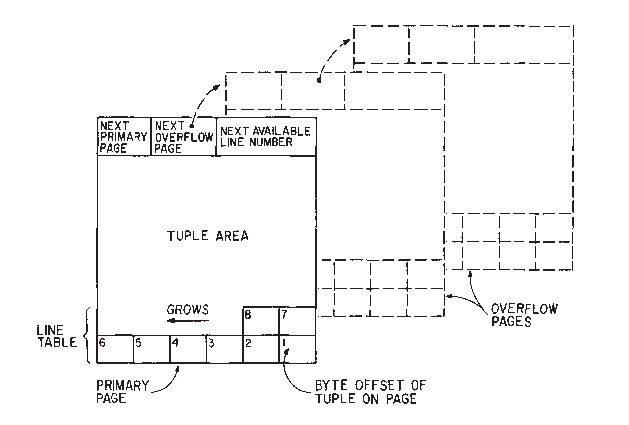
\includegraphics[height=66mm]{hayamiz/images/page-layout-ingres.eps}
  \caption{INGRESのページ構造}
  \label{174456_16Jul12}
 \end{center}
\end{figure}


{\bf ハッシュ}と{\bf ISAM}は,検索キーを用いて少量のタプルに対するアクセ
スを高速に行うことを可能とする構造です。{\bf ハッシュ}はハッシュテーブル
を使って,{\bf ISAM}は探索木を使って,検索キーとタプルIDの関連付けを行う
ことで高速なアクセスを実現しています。INGRESでは,タプルIDは (ページ番号,
ページ内ライン番号) という値のペアによって表現されているので,タプルIDさ
えわかれば目的のデータの在り処がわかります。


ページの構造は図\ref{174456_16Jul12}のようになっています。ページの先頭に
はヘッダ情報があり,またページの末尾にはラインテーブルと呼ばれるデータが
格納されています。ラインテーブルの各要素は,タプルのデータがページ内のど
の位置にあるかのオフセット情報を保持しています。タプルIDに含まれているペー
ジ内ライン番号は,このラインテーブル内のインデックス番号となっているので,
タプルIDさえわかればタプルのデータがどこにあるのかがわかるようになってい
ます。この構造には,タプルの物理的な位置が変化しても,ラインテーブルを更
新するだけで,タプルIDは変化することがないという利点があります。


\subsubsection{アクセスメソッドまとめ}


\begin{figure}
 \begin{center}
  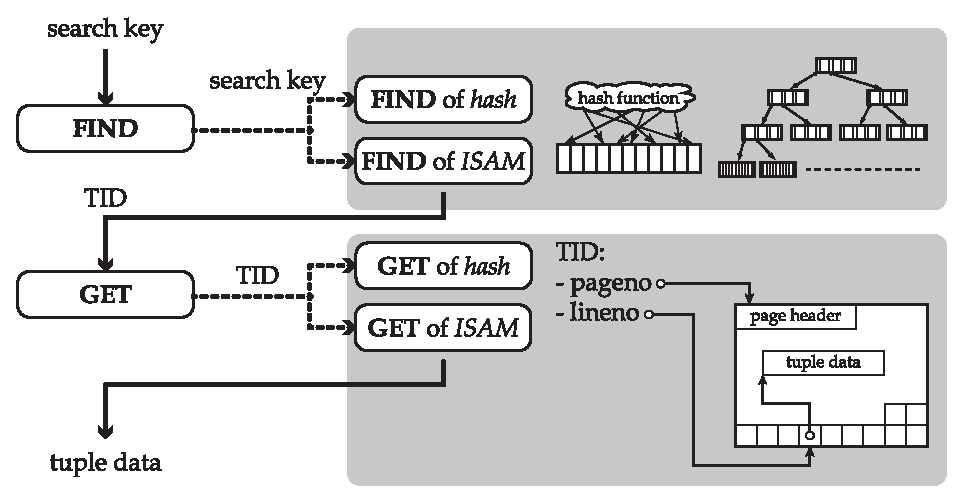
\includegraphics[width=100mm]{hayamiz/images/access-method.eps}
  \caption{検索キーを用いたアクセスメソッドによるタプルデータの取得}
  \label{190817_16Jul12}
 \end{center}
\end{figure}


検索キーが与えられてから,タプルのデータが得られるまでの一連の流れを図
\ref{190817_16Jul12}にまとめました。まずは検索キーが与えられると,{\bf
FIND}を呼び出してタプルIDを取得します。{\bf FIND}の中では,ハッシュテーブ
ルや木構造を用いて効率的にタプルIDの検索が行われます。そして,得られたタ
プルIDを引数として{\bf GET}を呼び出すことで,ページを読み出し,タプルのデー
タが取得されます。


この基本的なデータアクセスの枠組みは,INGRESの頃に確立され,現在でも殆ど
変わること無く引き継がれています。


ただ1980年頃まで,INGRESには B$^+$-tree を用いたアクセスメソッドは実装さ
れていませんでした。ISAMとB$^+$-treeはよく似ているのですが,根本的な違い
としてISAMは静的なアクセスメソッドであるのに対し,B$^+$-treeは動的なアク
セスメソッドであるということです。どちらも多分木構造を索引として用いてい
ますが,ISAMではデータの挿入や削除のたびに木構造を変更することはなく,適
当なタイミングでまとめて木構造を作り直します。そのため,頻繁にデータの挿
入,削除が行われる場合にはどんどん構造劣化が進み,アクセス性能が落ちてし
まいますが,参照が非常に多い場合には良い性能を発揮します。一方,
B$^+$-treeはデータの挿入,削除のたびに木構造を動的にバランスさせるために,
ISAMで起きるような構造劣化は起きません。しかし,1回の処理あたりのオーバー
ヘッドはISAMよりも大きくなってしまいます。


INGRESの開発において,何度もB$^+$-treeの導入が検討され,その度に採用が見
送られてきたようです。しかしながら,1980年のINGRES開発を振り返る論文にお
いて,StonebrakerはB$^+$-treeの採用を見送ってきたのは ``major mistakes''
の一つであり,次にアクセスメソッドを再検討する際にはB$^+$-treeも実装する
であろうと述べています。


また,INGRESのアクセスメソッドはUNIXのファイルシステムの上に構築されてい
たのですが,UNIXのファイルシステムによるオーバーヘッドが当初予測していた
よりも深刻なものであり,独自のファイルシステムを実装するべきであった,と
も同論文では述べられています。実際に,3年後に発表された論文において
Stonebraker 達は独自に実装したファイルシステムを使った場合と性能比較を行っ
ており,最大で70\%程度性能が向上することを確認しています。このように
INGRESの開発過程で得られた知見は,UNIXの開発にフィードバックされ,その発
展に大きく貢献しました。


\subsection{人材育成の場としてのINGRES}


INGRESプロジェクトは,初期のリレーショナルデータベース実装における技術を
確立するという非常に重要な功績を成し遂げました。しかし,INGRESプロジェク
トの功績はそれだけにとどまりません。後のデータベース業界を牽引する人材を
輩出したという点においても,その価値が評価されています。


INGRESプロジェクトの最初のチーフプログラマを務めた Gerald Held はTandem
Computers において NonStop SQL の開発に携わります。また別の時期にチーフプ
ログラマを務めた Robert Epstein は Sybase 社を設立してSybase の開発を行い
ます。また Peter Krepps はINGRES商用化に際して立ち上げられた Relational
Technology 社でプログラマとして活躍しました。


\section{System R}


INGRESプロジェクトからすこし遅れて,IBMでもリレーショナルデータベースシス
テム System R の研究開発が始まります。リレーショナルモデルの父である
Codd がIBMで働いていたにも関わらず,歴史を振り返るとIBMはリレーショナルデー
タベースシステム開発において常に後塵を拝しています。


当時のIBMではIMSが圧倒的な商業的成功を収めていました。そのため,IMSの開発
のために多くの投資を行っているIBMとしては,よくわからない数学で記述された
リレーショナルモデルは注目に値しないものだと思われたのでしょう。そのため,
リレーショナルモデルにもとづくデータベースシステムとしてSysmte Rの研究開
発が始まっても,スタッフとしては10人程度しか人員が配置されなかったようで
す。


IMSがベースとする階層型モデルはナビゲーショナルなので,プログラマがデータ
アクセスの方法を記述しなければなりませんでした。しかし見方を変えると,デー
タベースのことを熟知しているプログラマにとっては,最善の方法でデータアク
セスを行うことができるということでもあります。一方,リレーショナルモデル
ではプログラマが明示的にデータアクセスの方法を制御できません。究極的なパ
フォーマンスの観点からすると,ナビゲーショナルモデルが優位なのは確かです。
実際に,究極の性能が求められるミッションクリティカルなシステムでは,未だ
にナビゲーショナルデータベースシステムが用いられているようです
\footnote{JALのシステムにもIMSが使われているとか}。


その後,リレーショナル陣営とナビゲーショナル陣営は激しい論争を繰り広げて
ゆきますが,次第に世の中の流れはリレーショナルモデルに傾いてゆきました。
歴史を振り返ると,今やアセンブラを直接書くことが殆どないように,コンピュー
タの性能が良くなるにつれて技術のトレンドが変化するというのはままあること
です。データベースシステムにおいても,最初は性能が低くて受け入れられない
と思われていたリレーショナルモデルが,その利便性が故に主流となってゆきま
した。


\section{エピローグ}


1970年代,Coddによるリレーショナルモデルの提唱に始まり,INGRESやSystem R
の研究によってリレーショナルデータベースシステムが実用に耐えうるものであ
ることが証明されました。1981年には,Coddはその功績を認められ計算機科学分
野において最も権威あるチューリング賞を受賞します。


そして1970年代の終盤から1980年代は,商用リレーショナルデータベースシステ
ムが次々と登場し,熾烈な戦いを繰り広げてゆきます。


1977年,現在の Oracle の前身である Software Development Laboratories が
Larry Ellison と Robert Miner によって設立され,1979年には世界初のSQLベー
スの商用リレーショナルデータベースシステム Oracle RDBMS をリリースします。


1979年,Jack Shemer,Philip Neches,Walter Muir,Jerold Modes,William
Worth,Carroll ReedによってTeradataが設立され,1984年に世界初の並列データ
ベースシステムDBC 1012\footnote{ちなみに1012というのは$10^{12} = 1 \mathrm{TB}$にちなんでつけられた名前です}をリリースします。


1980年,Lawrence Rowe,Michael Stonebraker,Eugene Wong,Gary
Morgenthaler によって INGRES 商用化のために Relational Technology (後の
Ingres Corp.)が設立され,翌1981年に商用INGRESをリリースします。一方,UC
Berkeley においても INGRES プロジェクトは継続しており,こちらのほうは
University INGRES と呼ばれるようになります。University INGRES のソースコー
ドは現在UC Berkeleyのウェブサイトからダウンロード可能です\footnote{\verb|http://s2k-ftp.cs.berkeley.edu/ingres/|}。


時を同じくして,Roger Sippl と Laura King によって 1980年に Relational
Database Systems (後の Informix Software) が設立され,翌1981年に
Informix がリリースされます。


IBMは1981年にSQL/DSを,さらに1983年にはDB2をリリースしてリレーショナルデー
タベース市場に乗り出します。エンタープライズ市場の覇者であるIBMのこの動き
は,旧来のナビゲーショナルデータベースシステムに対する新興勢力リレーショ
ナルデータベースシステムの勝利を決定的なものにします。


1984年,Mark Hoffman,Bob Epstein,Jane Doughty,Tom Hagginによって
Sybaseが設立され,1986年にリレーショナルデータベースシステムSybaseをリリー
スします。後にSybaseはMicrosoftと提携してSybase SQL Serverを開発しました。
その設計は現在のMicrosoft SQL Serverにも受け継がれています。


同1984年,ミニコンピュータ市場を牽引するDECがOpenVMSオペレーティングシス
テムにおける機能として DEC Rdb を発表します。


1986年,無停止コンピュータシステムを主な事業として手がける Tandem
Computers が NonStop SQL をリリースします。


そして1990年代には更にプレイヤーが増えつつもその統廃合が進み,オブジェク
ト指向データベースシステムなど新興技術の登場,オープンソースのデータベー
スシステム隆盛の兆候など,データベースシステムは新たな時代へと突入してゆ
きます。


\section*{参考文献}


\small


\begin{itemize}
 \item E. F. Codd, ``A Relational Model of Data for Large Shared Data
       Banks'', {\it Communications of the ACM}, Volume 13, Number 6,
       1970
 \item E. F. Codd, ``A data base sublanguage founded on the relational
       calculus'', {\it Proceedings of the 1971 ACM SIGFIDET workshop
       on Data Description, Access and Control}, 1971
 \item C. J. Date, E. F. Codd, ``The relational and network approaches: Comparison of the
       application programming interfaces'', {\it Proceedings of the
       1974 ACM SIGFIDET workshop on Data Description, Access and
       Control}, 1975
 \item G. Held, M. Stonebraker, E. Wong, ``INGRES--A relational data
       base management system'', {\it Proceedings of AFIPS 1975 NCC},
       Volume 44, 1975
 \item M. Stonebraker, G. Held, E. Wong, P. Kreps, ``The design and
       implementation of INGRES'', {\it ACM Transactions on Database
       Systems}, Volume 1, Issue 3, 1976
 \item G. Held, M. Stonebraker, ``B-trees re-examined'', {\it Communications of the
       ACM}, Volume 21, Issue 2, 1978
 \item M. Stonebraker, ``Retrospection on a database system'', {\it ACM
       Transactions on Database Systems}, Volume 5, Issue 2, 1980
 \item D. Chamberlin, M. Astrahan, M. Blasgen, J. Gray, W. F. King,
       B. Lindsay, R. Lorie, J. Mehl, T. Price, F. Putzolu, P. Selinger,
       M. Schkolnick, D. Slutz, I. Traiger, B. Wade, R. Yost, ``A
       history and evaluation of System R'', {\it Communications of the
       ACM}, Volume 24, Issue 10, 1981
 \item M. Stonebraker, J. Woodfill, J. Ranstrom, M. Murphy, M. Meyer,
       E. Allman, ``Performance enhancements to a relational database
       system'', {\it ACM Transactions on Database Systems}, Volume 8,
       Issue 2, 1983
 \item Relational Technology Inc., ``INGRES The Distributed SQL
       Relational Database System Press Kit'', 1987
 \item National Research Council, ``Funding a Revolution: Government
       Support for Computing Research'', Natl Academy Pr, 1999
 \item M. Stonebraker, J. M. Hellerstein, ``What Goes Around Comes
       Around'', {\it Readings in Database Systems, Fourth Edition},
       Morgan Kaufmann, 2005
 \item A. Ances, ``RDBMS Workshop: Ingres and Sybase'', Computer
       History Museum, 2007
\end{itemize}


and so many online resources


\normalsize